% ============================================================
%  深圳大学实验报告模板（SZU Experiment Report Template）
%  Adapted for Project 1: NumPy 实现的 OpenCLIP ViT-B-32 图像编码器
%  Produced by: Chao Fan and Kewei Ou, AI School of SZU
% ============================================================

\documentclass[a4paper,12pt]{article}

% ----------------------------
% 中文与字体支持
% ----------------------------
\usepackage{fontspec}
\usepackage{xeCJK}
% 优先使用 Overleaf 自带的 Noto 字体；本机预览时回退到项目内附带的宋体
\IfFontExistsTF{Noto Serif CJK SC}{
    \setCJKmainfont{Noto Serif CJK SC}
}{
    \setCJKmainfont[
        Path=fonts/,
        Extension=.otf,
        UprightFont=SongtiSC-Regular,
        BoldFont=SongtiSC-Bold
    ]{SongtiSC-Regular}
}

% ----------------------------
% 页面设置与常用宏包
% ----------------------------
\usepackage{geometry}
\geometry{left=1in, right=1in, top=1in, bottom=1in}

\usepackage{longtable}
\usepackage{graphicx}
\usepackage{fancyhdr}
\usepackage{tikz}
\usetikzlibrary{calc}
\usepackage{verbatim}
\usepackage{float}
\usepackage{amsmath}
\usepackage{booktabs}
\usepackage{listings}
\usepackage{xcolor}
\usepackage[colorlinks=true,linkcolor=blue,urlcolor=blue]{hyperref}

% 代码样式
\lstset{
  basicstyle=\ttfamily\footnotesize,
  breaklines=true,
  frame=single,
  rulecolor=\color{gray!40},
  numbers=left,
  numberstyle=\tiny\color{gray},
  language=Python,
  keywordstyle=\color{blue},
  commentstyle=\color{green!40!black},
  showstringspaces=false
}

% ----------------------------
% 页眉页脚设置
% ----------------------------
\fancyhf{}
\fancyhead[C]{}
\fancyhead[R]{}

% ============================================================
%                      文档开始
% ============================================================

\begin{document}

% ============================================================
% 封面页
% ============================================================
\begin{titlepage}
    \centering
    \vspace*{2cm}
    \Huge{\textbf{深 \ 圳 \ 大 \ 学 \ 实 \ 验  \ 报 \ 告}}\\[1.5cm]

    {\Large\textbf{课程名称}\quad\underline{\makebox[8cm][c]{Python程序设计}}}\\[0.5cm]
{\Large
\noindent\makebox[3.2cm][l]{\textbf{项目名称}}
\underline{\makebox[8cm][c]{基于 NumPy 的 OpenCLIP ViT-B-32 图像编码器}}}\\[0.5cm]
{\Large
\noindent\makebox[3.2cm][l]{\textbf{学 \quad \quad 院}}
\underline{\makebox[8cm][c]{人工智能学院}}}\\[0.5cm]
{\Large
\noindent\makebox[3.2cm][l]{\textbf{专 \quad \quad 业}}
\underline{\makebox[8cm][c]{}}}\\[0.5cm]
{\Large
\noindent\makebox[3.2cm][l]{\textbf{指导教师}}
\underline{\makebox[8cm][c]{舒婷}}}\\[0.5cm]
{\Large
\noindent\makebox[3.2cm][l]{\textbf{报 \quad 告 \quad 人}}
\underline{\makebox[3cm][c]{}}
\hspace{0.5cm}
\textbf{学号}
\underline{\makebox[3cm][c]{}}}\\[0.5cm]
{\Large
\noindent\makebox[3.2cm][l]{\textbf{实验时间}}
\underline{\makebox[8cm][c]{}}}\\[0.5cm]
{\Large
\noindent\makebox[3.2cm][l]{\textbf{提交时间}}
\underline{\makebox[8cm][c]{}}}\\[1.5cm]

    \vfill
    \Large{\textbf{教务处制}}
\end{titlepage}

\newpage

% ============================================================
% 正文部分
% ============================================================

% ----------------------------
\section{实验目的 Objectives}

本实验要求在不使用 PyTorch、OpenCLIP 等深度学习框架的前提下，仅使用 NumPy 复现 OpenCLIP
ViT-B-32 图像编码器的\textbf{前向计算}。具体目标包括：

\begin{enumerate}
    \item[1.] 理解 Vision Transformer (ViT) 的图像分块（patchify）、线性投影、位置编码、
        多头自注意力（Multi-Head Self-Attention）与前馈网络（MLP）的完整计算流程；
    \item[2.] 用 NumPy 的数组操作（reshape/transpose、矩阵乘法、规约、广播）实现六个核心环节
        （TODO-01 $\sim$ TODO-06），输出必须在数值上与给定的 FP32 参考结果一致；
    \item[3.] 通过分阶段数值校验，保证中间张量（patches、input tokens、block0、last tokens）
        与最终输出 token 均满足给定的误差容限；
    \item[4.] 该编码器将作为期末项目 \texttt{szu\_python\_openclip} 的图像塔（image tower）
        被复用，因此必须保持与最终项目一致的类接口。
\end{enumerate}

% ----------------------------
\section{实验内容概述 Overview}

模型的整体数据流如图~\ref{fig:pipeline} 所示。输入为经过预处理的 float32 图像批次
$[B,3,224,224]$，依次经过图像分块、patch 投影、CLS 拼接与位置编码、12 个 Transformer
块、后归一化，最后选取 CLS token 投影并做单位长度缩放，得到每张图像一行归一化的输出 token
$[B,512]$。全部 152 个视觉参数张量由 \texttt{weights/image\_encoder.npz} 提供，实验过程中
\textbf{不进行任何参数更新}。

\begin{figure}[H]
    \centering
    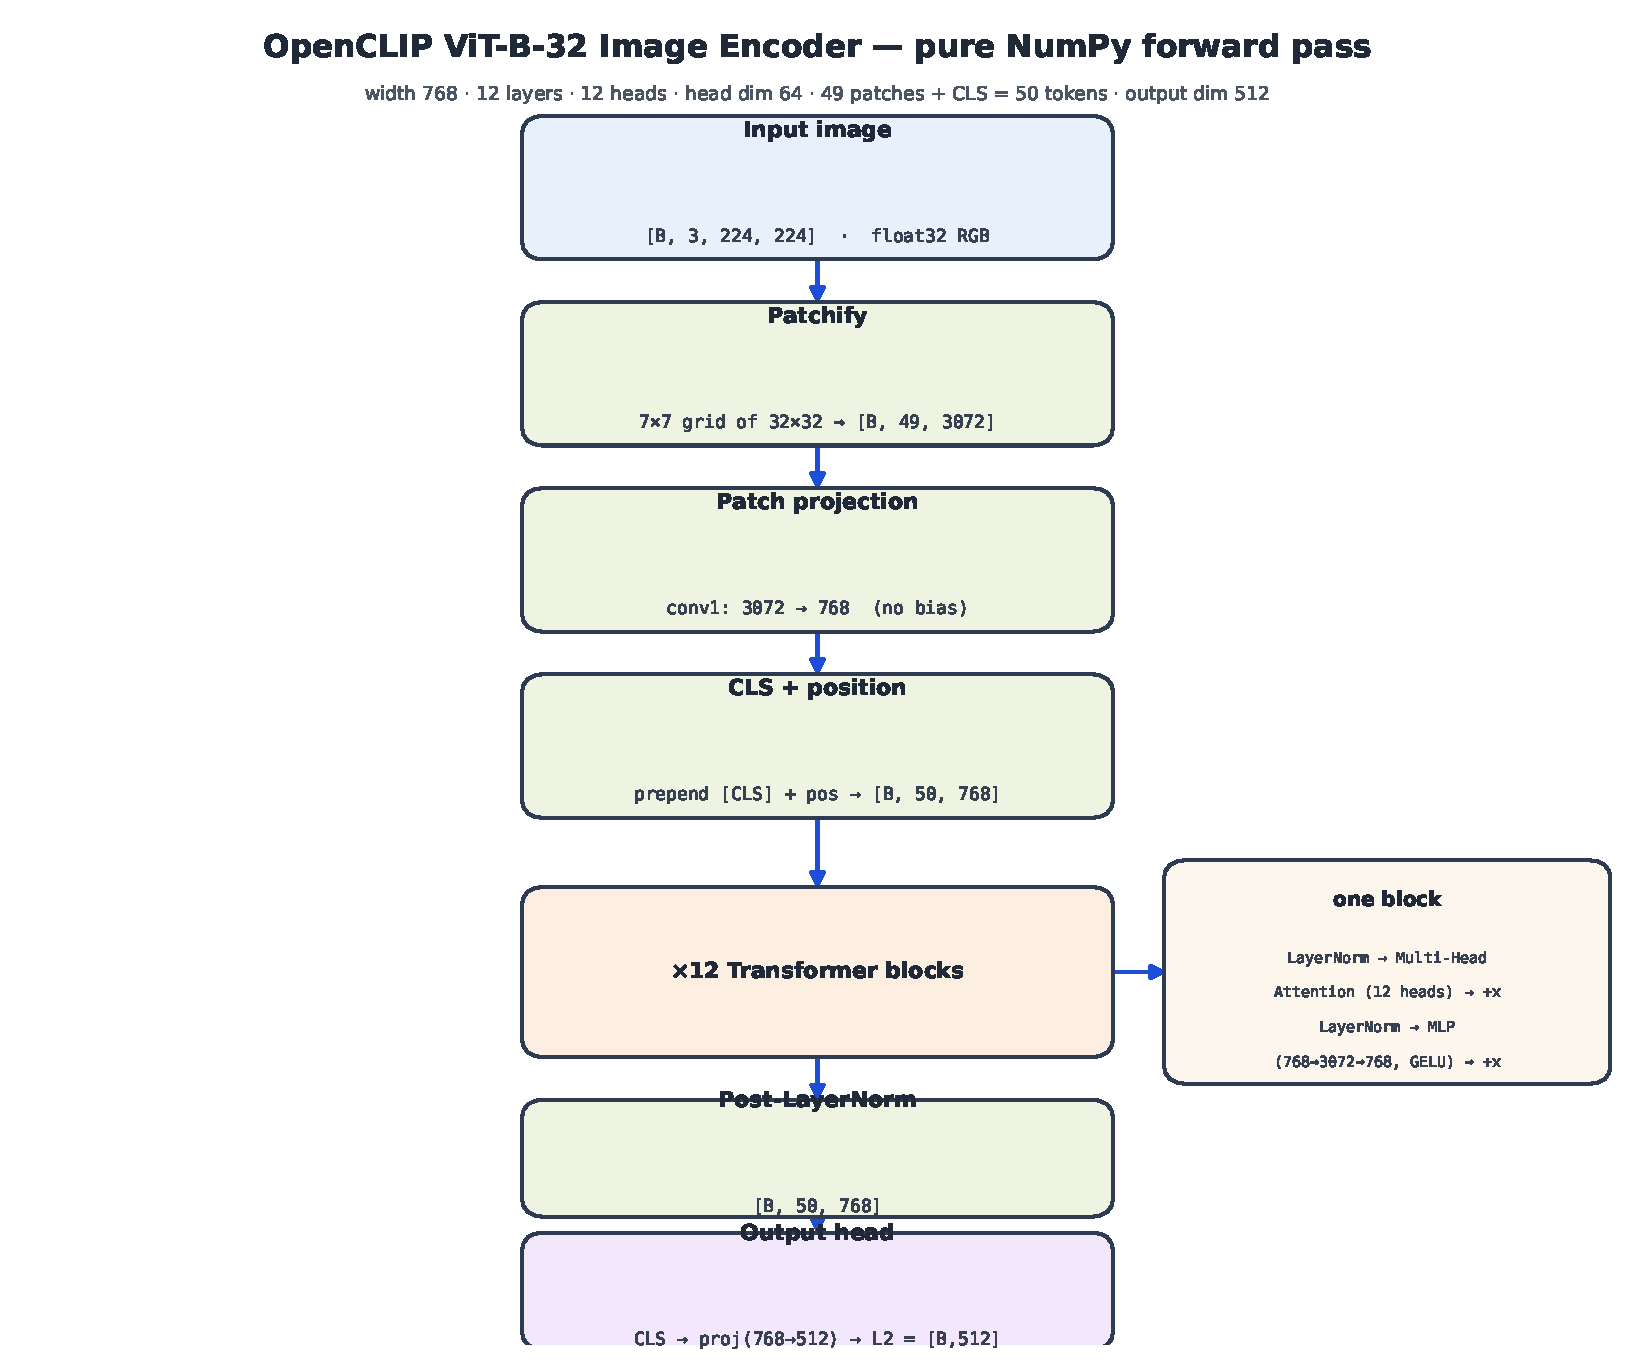
\includegraphics[width=0.92\linewidth]{figs/image_encoder_pipeline.pdf}
    \caption{OpenCLIP ViT-B-32 图像编码器的前向计算流程}
    \label{fig:pipeline}
\end{figure}

主要实现要点如下：
\begin{enumerate}
    \item[Patch 嵌入:] 将 $224\times224$ 图像切成 $7\times7$ 个 $32\times32$ 的 patch，每个 patch
        展平成 3072 维行向量，再经无偏置线性投影映射到 768 维；
    \item[多头注意力:] 每个 block 内先做 LayerNorm，再计算 12 个注意力头的 q/k/v、缩放点积分数、
        softmax 系数与加权求和，合并各头后做输出投影；
    \item[残差与 MLP:] 注意力更新与 MLP 更新各自与输入做残差相加，MLP 使用精确 GELU 激活；
    \item[输出头:] 选取第 0 号 CLS token，经后归一化与 $768\to512$ 投影，最后做 L2 归一化。
\end{enumerate}

% ----------------------------
\section{实现细节 Implementations}

\subsection{图像分块与投影（TODO-01 / TODO-05）}

分块的关键在于把图像重排为 patch 网格后展平，顺序保持“先从左到右、再从上到下”，
每个 patch 内部按 $C,H,W$ 顺序展平：

\begin{lstlisting}
B, C, H, W = images.shape
grid = H // 32                    # 7
x = images.reshape(B, C, grid, 32, grid, 32)   # [B,C,7,32,7,32]
x = x.transpose(0, 2, 4, 1, 3, 5)              # [B,7,7,C,32,32]
patches = x.reshape(B, grid*grid, C*32*32)     # [B,49,3072]
patches = patches @ self.patch_weight.T        # [B,49,768] (no bias)
\end{lstlisting}

随后把学习到的 CLS 行拼接到 token 轴最前面，再加上可广播的位置编码，得到
$[B,50,768]$ 的输入 token 序列。

\subsection{多头自注意力（TODO-02 / TODO-03）}

将 $D=768$ 的特征轴拆成 $H=12$ 个头，每头 $64$ 维：

\begin{lstlisting}
B, N, D = x.shape
x = x.reshape(B, N, self.heads, self.head_dim) # [B,N,H,64]
x = x.transpose(0, 2, 1, 3).reshape(B, self.heads, N, self.head_dim)
\end{lstlisting}

注意真实的 $k$ 是四维张量，转置时\textbf{只交换最后两轴}，保持 batch 与 head 分组不变：

\begin{lstlisting}
kt = k.transpose(0, 1, 3, 2)                    # [B,H,64,N]
scores = (q @ kt) / np.sqrt(np.float32(self.head_dim))
coefficients = attention_weights(scores)       # supplied softmax helper
context = coefficients @ v                     # [B,H,N,64]
merged = context.transpose(0, 2, 1, 3).reshape(B, N, self.width)
return merged @ self.out_weight.T + self.out_bias   # [B,N,768]
\end{lstlisting}

\subsection{Transformer 块（TODO-04）}

每个块包含两条残差路径：

\begin{lstlisting}
update  = self.attention(self.norm1(x))   # attention update
residual = x + update                     # 1st residual
u = self.norm2(residual)                  # 2nd LayerNorm
hidden = self.gelu(u @ self.fc1_weight.T + self.fc1_bias)   # [B,N,3072]
mlp_update = hidden @ self.fc2_weight.T + self.fc2_bias     # [B,N,768]
return residual + mlp_update              # 2nd residual
\end{lstlisting}

所有存储的线性层权重均为 $[\text{out},\text{in}]$ 布局，因此矩阵乘前需要转置；唯一例外是
\texttt{visual.proj}，它已是 $[768,512]$ 的 $[\text{in},\text{out}]$ 布局，直接使用即可。

\subsection{输出头（TODO-06）}

\begin{lstlisting}
cls = tokens[:, 0, :]                    # select CLS: [B,50,768] -> [B,768]
output = self.post_norm(cls) @ self.projection   # [B,512]
return unit_vector(output)               # supplied L2 normalization
\end{lstlisting}

% ----------------------------
\section{实验结果 Results}

运行 \texttt{python check.py --stage all}，全部 8 个阶段（含资产校验）均通过。各阶段的
数值误差如下（内部 token 容差 \texttt{atol=2e-4, rtol=2e-4}；输出 token 容差
\texttt{atol=2e-5, rtol=2e-4}；预处理 \texttt{atol=2e-6}）：

\begin{table}[H]
\centering
\begin{tabular}{lccc}
\toprule
阶段 Stage & 形状 Shape & 最大绝对误差 max\_abs & 平均绝对误差 mean\_abs \\
\midrule
preprocess   & $(10,3,224,224)$ & $0.0$          & $0.0$          \\
patches      & $(2,49,3072)$    & $0.0$          & $0.0$          \\
tokens       & $(2,50,768)$     & $0.0$          & $0.0$          \\
block0       & $(2,50,768)$     & $7.540\times10^{-6}$ & $2.274\times10^{-7}$ \\
last\_tokens & $(2,50,768)$     & $4.387\times10^{-5}$ & $2.406\times10^{-6}$ \\
output       & $(10,512)$       & $6.780\times10^{-7}$ & $8.215\times10^{-8}$ \\
batch        & $(3,512)$        & $4.619\times10^{-7}$ & $8.133\times10^{-8}$ \\
\bottomrule
\end{tabular}
\caption{分阶段数值校验结果（全部 PASS）}
\label{tab:errors}
\end{table}

可以看到，patch 切分、token 拼接等纯索引/重排操作误差为\textbf{精确 0}；进入矩阵乘法后误差
随层数缓慢累积，但最终输出 token 的最大绝对误差仅为 $6.78\times10^{-7}$，远小于
$2\times10^{-5}$ 的容限，说明实现与独立 FP32 参考完全吻合。

% ----------------------------
\section{讨论与总结 Discussion}

\subsection{一次形状变换（shape change）}

最关键的形状变换出现在 \texttt{patchify}：输入 $[B,3,224,224]$ 需要变成 $[B,49,3072]$。
如果直接 reshape 会打乱 patch 顺序，正确做法是先把空间维度拆成网格轴
$[B,3,7,32,7,32]$，再用 \texttt{transpose(0,2,4,1,3,5)} 把网格轴 $(7,7)$ 提到前面、
通道与像素轴放到后面，最后展平。这一变换同时满足了“先左后右、先上后下”的 patch 顺序和
“$C,H,W$”的展平顺序。

\subsection{一个修复的 bug}

初版代码中缩放因子写作 \texttt{np.sqrt(self.head\_dim)}，由于 \texttt{head\_dim} 是 Python
整数，\texttt{np.sqrt} 返回 float64 标量，导致 \texttt{scores} 被隐式提升为 float64，
校验阶段报错 \texttt{block0: use float32}。修复方式是把标量显式转为 float32：
\texttt{np.sqrt(np.float32(self.head\_dim))}，此后所有阶段均保持 float32 并通过校验。

\subsection{其它说明}

在 macOS 上使用 NumPy 的 BLAS 后端（Accelerate/vecLib）进行 float32 矩阵乘法时，会打印
``divide by zero / invalid value encountered in matmul'' 一类的\textbf{误报警告}，但结果
有限且正确。该现象来自底层 BLAS 库，与本实现无关，可在运行时忽略。

\subsection{贡献与协助}

本实验由本人独立完成：六个 TODO 环节的实现、调试与数值校验均由本人完成。学习过程中参考了
课程讲义（第 39--76 页）与配套教学脚本 \texttt{transformer\_steps.py}，以及附件中提供的
\texttt{helpers.py} 数值辅助函数与起始框架代码。

\subsection{代码仓库与复现}

完整代码、复现说明（README）与运行结果均已上传至 GitHub：
\url{https://github.com/your-username/your-repo}。
在仓库根目录依次执行以下命令即可复现全部结果：

\begin{lstlisting}
python -m pip install -r requirements.txt
python check.py --stage all        # staged numerical checks
python run.py --output output_tokens.npz   # write output tokens
\end{lstlisting}

\subsection{总结}

本实验完整地复现了 ViT-B-32 图像编码器的 NumPy 前向计算，全部 8 个校验阶段一次性通过，
且输出误差稳定在 $10^{-6}\sim10^{-7}$ 量级。通过手写矩阵乘法、转置与广播，我对多头注意力的
头组织方式、两层残差连接与 LayerNorm 的逐元素计算有了更直观的理解，为期末项目
\texttt{szu\_python\_openclip} 的图像塔实现打下了基础。

\newpage

% ============================================================
% 批阅与成绩评定页
% ============================================================

\begin{tikzpicture}[remember picture, overlay]
  \draw[thick]
    ($(current page.north west)+(2cm,-3cm)$)
    rectangle
    ($(current page.south east)+(-2cm,3.5cm)$);
\end{tikzpicture}

\vspace{1cm}

\noindent \textbf{指导教师批阅意见：}
\vspace{6cm}
\hfill

\vspace{1cm}

\noindent \textbf{成绩评定：}
\vspace{2cm}
\hfill

\vspace{1cm}

\noindent
\hfill
\textbf{指导教师签字：}\quad\quad\quad\quad\quad\\[0.5cm]

\hfill
\textbf{年}\quad\quad
\textbf{月}\quad\quad
\textbf{日}\quad

\vspace{1cm}

\noindent \textbf{备注：}

\begin{tikzpicture}[remember picture, overlay]
  \node[
    anchor=north west,
    inner sep=0pt,
    text width=\dimexpr\paperwidth-4cm\relax
  ] at ($(current page.south west)+(2cm,3.1cm)$) {
    \begin{minipage}{\dimexpr\paperwidth-4cm\relax}
      \small
      \noindent
      \textbf{注：}\;1、报告内的项目或内容设置，可根据实际情况加以调整和补充。\\[0.2cm]
      \phantom{\textbf{注：}\;}2、教师批改学生实验报告时间应在学生提交实验报告时间后 10 日内。
    \end{minipage}
  };
\end{tikzpicture}

% ============================================================
%                      文档结束
% ============================================================

\end{document}
